\documentclass{standalone}
\usepackage{pgfplots}
\usetikzlibrary{decorations.pathreplacing}

\begin{document}
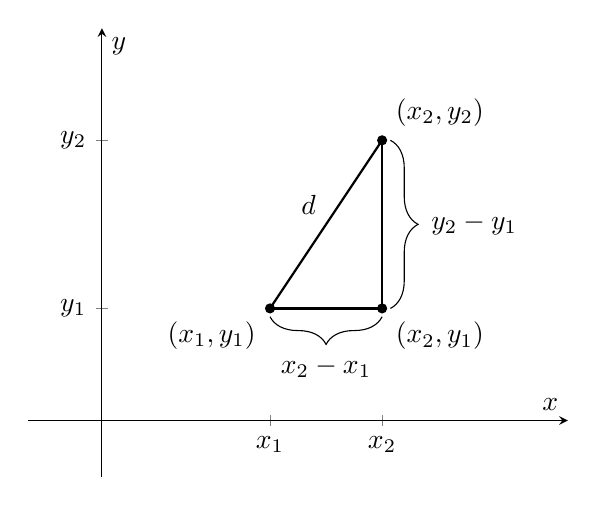
\begin{tikzpicture}
  \begin{axis}[
    axis equal,
    axis lines=middle,
    xmin=-1,xmax=8,
    ymin=-1,ymax=7,
    xlabel=\(x\),
    ylabel=\(y\),
    xtick={3,5},xticklabels={\(x_1\),\(x_2\)},
    ytick={2,5},yticklabels={\(y_1\),\(y_2\)}
    ]
    \node[label={215:{\((x_1,y_1)\)}},circle,fill,inner sep=1.3pt] at (axis cs:3,2) {};
    \node[label={45:{\((x_2,y_2)\)}},circle,fill,inner sep=1.3pt] at (axis cs:5,5) {};
    \node[label={315:{\((x_2,y_1)\)}},circle,fill,inner sep=1.3pt] at (axis cs:5,2) {};
    \draw[thick] (axis cs:3,2) -- node[midway,above left] {\(d\)} (axis cs:5,5);
    \draw[thick] (axis cs:3,2) -- (axis cs:5,2) -- (axis cs:5,5);
    % brace to indicate length of base
    \draw[decorate,decoration={brace,amplitude=10pt,mirror,raise=3pt}]
    (axis cs:3,2) -- node[midway,below,yshift=-0.5cm] {\(x_2-x_1\)} (axis cs:5,2);
    % brace to indicate length of side
    \draw[decorate,decoration={brace,amplitude=10pt,mirror,raise=3pt}]
    (axis cs:5,2) -- node[midway,right,xshift=0.5cm] {\(y_2-y_1\)} (axis cs:5,5);
  \end{axis}
\end{tikzpicture}
\end{document}
